% Chapter Template

\chapter{Sistema d'adaptabilitat} % Main chapter title

\label{DissenySistema} % Change X to a consecutive number; for referencing this chapter elsewhere, use \ref{ChapterX}

Els models UML prèviament descrits ens permeten dissenyar i modelar de forma estandarditzada el sistema de monitoratge. Proporciona, semànticament, tots els recursos necessaris per traduir propostes de configuracions de sistemes en accions reals sobre els monitors implementats.\\

El següent pas és el disseny i implementació d'un sistema que, a partir dels models anteriors, i de tot el domini que defineixen, sigui capaç de gestionar la persistència dels models, obtenir-ne els necessaris per aplicar reconfiguracions, actualitzar els models d'acord a aquestes modificacions, i traduir la informació implícita als models en accions de reconfiguració reals a enviar al sistema de monitoratge.\\

Procedirem a presentar els diferents components que componen aquest sistema.

\section{Model Repository}

El primer component que cal introduir per començar a entendre el \textit{workflow} del sistema d'adaptabilitat és el \textbf{Model Repository}. Aquest component actua en termes genèrics com a un repositori que gestiona la persistència del conjunt de models UML que intervenen en el modelatge del sistema i la seva reconfiguració. Això, per tant, implica tot el conjunt de models descrits anteriorment: \textit{Base Model}, \textit{Feature Model}, \textit{Feature Configuration}, \textit{Pattern Model}, \textit{Profile Model} i \textit{Adaptability Model}.\\

Principalment, les funcionalitats que ha de satisfer són les següents:

\begin{enumerate}
\item Gestionar la persistència dels models en disc
\item Mapejar i encapsular l'estructura de directoris definida per estructurar els models segons el seu tipus
\item Encapsular els mètodes CRUD bàsics per la gestió dels models, aïllant la lògica interna de la resta de components
\item Encapsular mètodes extensius que permetin obtenir models sota unes certes característiques
\end{enumerate}

D'aquesta manera, podem concebre aquest component com una abstracció entre la naturalesa interna dels models i la lògica associada a la càrrega/descàrrega de fitxers amb el nostre sistema, assignant la responsabilitat d'aquests primers punts al Model Repository.\\

Una primera aproximació que ens podríem plantejar seria implementar un component unitari que definís un controlador (que després s'exposaria com a servei per integrar a IF) amb tots els mètodes necessaris per la gestió dels models. Si al nostre sistema únicament resultés d'interès les operacions bàsiques de models, aquesta seria una bona alternativa, ja que estaríem simplificant l'arquitectura del sistema, i hi hauria poc marge per la millora. Però si anem un pas més enllà, i plantegem les necessitats de reconfiguració i adaptabilitat del nostre sistema, veiem que un controlador basat en operacions CRUD únicament ens permetria definir reconfiguracions on tots els models que intervenen en l'adaptació són triats estàticament, no dinàmicament. És a dir: el potencial que oferiria el Model Repository seria referenciar els models implicats en una adaptació mitjançant els seus identificadors, que haurien de ser introduïts manualment.\\

Això per tant implica que no podríem aplicar escenaris d'adaptació com per exemple:\\

\centerline{Actualitzar el sistema de monitoratge amb la darrera Feature Configuration computada}\bigskip

Si tornem al cicle \textit{MAPE-k}, suposant un sistema de \textit{\textbf{P}lanificació} que produeix noves propostes de configuració (FC), aquest enviaria periòdicament aquests models al nostre sistema d'adaptabilitat. Si el nostre sistema és capaç de consultar les dates en què aquestes propostes es van afegint, és capaç de computar quina és la darrera afegida. I en definitiva, és capaç de computar, de forma automàtica i sense necessitat de donar-li cap mena d'informació, quins canvis aplicar al sistema de monitoratge.\\

Aquest escenari és clau pel nostre projecte. L'automatització del nostre sistema ve donada precisament gràcies a la persistència dels models UML i a l'actualització d'aquests, responsabilitat d'un altre sistema, a partir dels quals aquest és capaç de llegir, processar i traduir en modificacions reals sobre les activitats de monitoratge. Aquest escenari, però, és només un exemple de possible escenari d'adaptabilitat, basat en un criteri com la data, que serà el que nosaltres farem servir pel desenvolupament del projecte. Però el potencial està en veure que els criteris poden ser diversos, sempre i quan es treballin amb metadades que podem extreure a partir dels models, com és el cas de la data de generació de les propostes de reconfiguració.\\

Addicionalment a aquest problema, alguns models tenen dependències amb altres models UML. El cas més evident, l'\textit{Adaptability Model}, té dependències amb \textit{Feature Configurations}, que alhora tenen dependències amb \textit{Feature Models}, i també amb \textit{Pattern Models} i \textit{Profile Models}. La resolució i gestió d'aquestes dependències pot arribar a ser extremadament complicada si, al carregar un d'aquests models, necessitem computar i resoldre quines són aquestes dependències cada vegada que volem carregar el Model Repository a memòria per executar una adaptació des del component encarregat d'aquest aspecte, l'Adapter, que satisfent el criteri de distribució del nostre sistema pot no tenir accés al mateix repositori en disc que el Model Repository. \\

Partint d'aquestes necessitats, és evident que necessitem estendre els mètodes de lectura de models a mètodes més complerts, on utilitzem dades auxiliars per fer cerques dins el nostre repositori. És en aquest punt quan aquesta primera aproximació resulta ineficient: si volem accedir a les metadades dels fitxers dels models, tals com la data de creació, l'autor, el sistema que l'ha computat, etc. (més endavant les veurem amb més detall), carregar tots els fitxers dinàmicament per accedir a aquestes dades per fer la cerca resulta molt ineficient. És per això que, alternativament, utilitzarem la següent arquitectura per gestionar la persistència de models:

\begin{itemize}
\item \textbf{Model Repository Manager.} Component que gestiona les metadades dels models, emmagatzemades en una base de dades relacionals, i que estén un controlador amb els mètodes de cerca per obtenir els identificadors dels models associats.
\item \textbf{Model Repository Client.} Component que es comunica amb el Model Repository Manager per obtenir les dades dels models, gestiona la persistència del repositori de models, i encapsula els mètodes i objectes per obtenir i treballar amb els models associats a les reconfiguracions.
\end{itemize}

D'aquesta manera, el primer assumeix les responsabilitats de cerca i gestió de models en base a les seves metadades, i el segon assumeix la responsabilitat principal d'encapsular programàticament l'accés als models, per tal que la resta de components del sistema d'adaptabilitat puguin aïllar-se de la lògica interna d'aquest punt.

\subsection{Model Repository Manager}

Satisfent les necessitats del Model Repository Manager, necessitem contemplar els següents punts:

\begin{enumerate}
\item Disseny i implementació d'una base de dades relacional que emmagatzemi les metadades per cada tipus de model.
\item Disseny i implementació d'un component que accedeixi a la base de dades, i que exposi a través d'un controlador els mètodes de consulta i modificació dels models.
\end{enumerate}

\subsubsection{Disseny de la base de dades}

En primer lloc necessitem definir quines seran les metadades que considerarem per cada model. Generalment, podem considerar que tots els models definits tindran les següents dades:

\begin{itemize}
\item \textbf{Id.} Identificador d'aquell model, únic pel tipus de model (\textit{Base Model}, \textit{Feature Model}...) que representa.
\item \textbf{Name.} Nom del fitxer del model (sense l'extensió).
\item \textbf{AuthorId.} Identificador de l'autor del model.
\item \textbf{CreationDate.} Data de creació del model.
\item \textbf{LastModificationDate.} Data de la darrera modificació del fitxer del model.
\item \textbf{FileExtension.} Extensió del fitxer (.uml, .vql, .yamfc ...)
\item \textbf{SystemId.} Utilitzat dins el context SUPERSEDE per identificar els models que corresponen als diferents escenaris. En el nostre cas, aquest sempre serà \textit{MonitoringReconfiguration}.
\item \textbf{RelativePath.} Ruta relativa del directori \textit{root} on s'emmagatzema el model.
\item \textbf{Dependencies.} Llistat d'identificadors dels models dels quals depèn aquest model.
\end{itemize}

Tot i així, addicionalment existeix la possibilitat d'estendre atributs específics pels diferents models. Considerarem útils pel nostre context els següents:

\begin{itemize}
\item \textbf{Base Model}
\begin{itemize}
\item \textbf{Status.} Indica si el model ha estat computat per un sistema extern (\textit{ComputedByDM}) o bé si és el resultat d'una adaptació dins el sistema d'adaptabilitat (\textit{Enacted}).
\end{itemize}
\item \textbf{Feature Configuration}
\begin{itemize}
\item \textbf{Status.} Ídem que l'atribut al \textit{Base Model}
\end{itemize}
\item \textbf{Adaptability Model}
\begin{itemize}
\item \textbf{Feature Id.} Identificador de la \textit{feature} referenciada per l'Adaptability Model.
\end{itemize}
\end{itemize}

A partir d'aquestes dades podem procedir al disseny de la base de dades del repositori de metadades. Al existir atributs comuns i atributs diferenciats, hem de decidir quin tipus d'herència apliquem a la base de dades. Recordant les tres opcions, aplicades al nostre cas obtindríem el següent:

\begin{itemize}
\item \textbf{\textit{Single table inheritance.}} Definir una única taula a la base de dades \textit{Model} que inclogui tots els atributs possibles, inclosos els específics, i prengui valors nulls per aquells que no tenen aquell atribut.
\item \textbf{\textit{Class table inheritance.}} Definir una taula genèrica \textit{Model} i N taules addicionals per cada tipus que referenciïn la primera, amb els atributs addicionals per cada cas.
\item \textbf{\textit{Concrete table inheritance.}} Definir una taula per cada tipus de model i replicar els atributs comuns.
\end{itemize}

En el nostre cas, optarem per l'opció \textit{concrete table inheritance}. La raó principal d'aquesta opció és que, tot i compartir la major part de les dades, les entitats de models amb tipus diferents mai tindrà sentit contemplar-les conjuntament. És a dir: qualsevol lectura o modificació de models es farà sobre un model (o conjunt de models) d'un tipus específic, mai sobre models de forma genèrica (no tindrà sentit concebir l'entitat \textit{Model} abstracta). Si considerem la segona opció, veiem que seria molt ineficient, ja que caldria fer \textit{joins} internes per obtenir les dades els models, i per la mateixa raó que la ja esmentada sabem que seria un cost innecessari. Per tant, optarem per definir una taula per cada tipus, mantenint així la independència de les metadades entre models. A la figura ~\ref{fig:Figura20} podem veure el disseny proposat de la base de dades, d'acord als 6 tipus de models definits.\\

\begin{figure}
\centering
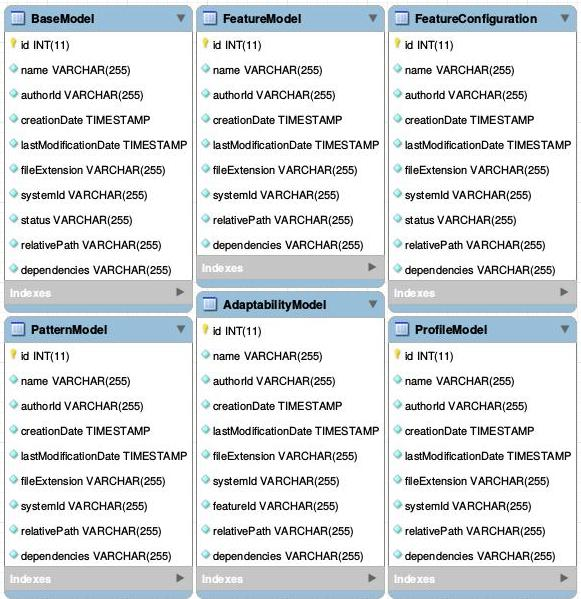
\includegraphics[width=13cm]{Figures/Figure20}
\decoRule
\caption{Disseny de la base de dades del Model Repository Manager}
\label{fig:Figura20}
\end{figure}

\subsection{Model Repository Client}

\section{Adapter}

\section{Model Adapter}

\section{Enactor}
